\documentclass{ctexart}
\setCJKmainfont{BabelStone Han}
\usepackage[natbibapa]{apacite}
\bibliographystyle{apacite}
\usepackage{fancyhdr}
\pagestyle{fancy}
\fancyhf{} % Clear all header and footer fields
\renewcommand{\footrulewidth}{0.4pt} % Optional: add a line above the footer
\fancyfoot[C]{This article is available at doi.org/10.6084/m9.figshare.25951900 \newline SAMIM KHALEQI 2024} % Change the text to whatever you want
% BASE TAKEN FROM ICCS315 SCRIBE NOTES

% --- SETUP STUFF ---
\usepackage[a4paper, margin=1in]{geometry}
\usepackage{enumitem}
\usepackage{booktabs}


\usepackage{url}
\usepackage[unicode]{hyperref}
\hypersetup{colorlinks=true,urlcolor=blue,citecolor=blue,linkcolor=red}

\usepackage{csquotes}
\usepackage{graphicx}

\setcounter{secnumdepth}{2}

\usepackage{titlesec,blindtext,color}

% --- MATH STUFF ---
\usepackage{amsthm, amsmath, amssymb}
\usepackage{mathtools,xspace}
\usepackage{nicefrac}

\usepackage{bbm}
\usepackage{dsfont}
\usepackage{cancel}

\usepackage{blkarray}
\newcommand{\matindex}[1]{\mbox{\scriptsize#1}} % Matrix index

% --- FONT STUFF ---
% Has to be under math stuff for some reason :/
\usepackage{newpxtext, newpxmath}
\usepackage[T1]{fontenc}

% --- DIAGRAM STUFF ---
\usepackage{tikz,pgfplots,xcolor,graphicx}
\usepackage{graphicx}
\usepackage{tabularx}
\usepackage{colortbl}
\usepackage{caption}
\usepackage{subcaption}

\usepackage[breakable,skins]{tcolorbox}
\usepackage{framed}
\usepackage{mdframed}
\usepackage{float}

\pgfplotsset{compat=1.18}

% --- THEOREM STUFF ---
\newtheorem{theorem}{Theorem}[section]
\newtheorem{proposition}[theorem]{Proposition}
\newtheorem{lemma}[theorem]{Lemma}
\newtheorem{corollary}[theorem]{Corollary}

\theoremstyle{definition}
\newtheorem{definition}[theorem]{Definition}
\newtheorem{example}[theorem]{Example}

\theoremstyle{remark}
\newtheorem{remark}[theorem]{Remark}
\newtheorem{claim}[theorem]{Claim}
\newtheorem{fact}[theorem]{Fact}

\usepackage{algorithm}
\usepackage[indLines=true]{algpseudocodex}
\usepackage{algorithmicx}
\algnewcommand\algorithmicinput{\textbf{Input:}}
\algnewcommand\Input{\item[\algorithmicinput]}
\algrenewcommand\algorithmicoutput{\textbf{Output:}}
\algrenewcommand\Output{\item[\algorithmicoutput]}
\algrenewcommand\algorithmicrequire{\textbf{Require:}}
\algrenewcommand\Require{\item[\algorithmicrequire]}

% --- CODE STUFF ---
\usepackage{minted}
\usemintedstyle{tango}

%=====================================================================================
% Define natbib-style citation commands - omitted uts prefix for ease of use
%=====================================================================================
\newcommand{\citep}{\parencite}
\newcommand{\citet}{\textcite}


%=====================
% Footnote
%=====================
\newcommand\utsnfootnotenumberless[1]{%
  \begingroup
  \renewcommand\thefootnote{}\footnote{#1}%
  \addtocounter{footnote}{-1}%
  \endgroup
}



%=====================================================================================
% Quotes and emphasis
%=====================================================================================
%=====================
% Quote - As a block of text
%=====================
\newcommand{\utsquote}[1]{
  \begin{quote}
    \input{partials/quotes/#1}   
  \end{quote}
}


%=====================
% Quote inline - Within a block of text
%=====================
\newcommand{\utsquoteinline}[1]{
  \input{partials/quotes/#1}
  \hspace*{-\parindent/2 + \parindent/10} % this is a hack to remove trailing white space
}


%=====================
% Definition - As a block of text
%=====================
\newcommand{\utsdefinition}[1]{
  \begin{quote}
    \input{partials/definitions/#1}   
  \end{quote}
}




%=====================
% Emphasise as a big text
%=====================
\newcommand{\utsemphbig}[1]{%
  \begin{center}
    {\fontsize{18}{22}\selectfont #1}
  \end{center}
}

%=====================
% Emphasise as a box
%=====================
\newmdenv[linecolor=gray,frametitle=,roundcorner=8pt]{utsinfobox}
\newcommand{\utsemphbox}[1]{
    \begin{utsinfobox}[backgroundcolor=gray!10]
        \emph{#1}
    \end{utsinfobox}
}


%=====================
% Emphasise as a box with title
%=====================
\newmdenv[linecolor=gray,
    shadow=true,
    shadowsize=1pt,
%    linewidth=1pt,
    frametitlerule=true,    
    roundcorner=10pt,
    backgroundcolor=gray!10]
    {utsshadowbox}    
\newcommand{\utsemphboxtitled}[2]{    
    \begin{utsshadowbox}[frametitle={#1}]
        \emph{#2}
    \end{utsshadowbox}
}



%===================== 
% Emphasis as horizontal lines above and below text
%=====================
\newcommand{\utsemphlines}[1]{
    \begin{center}
    \begin{itshape}
        \begin{tabular}{>{\centering\arraybackslash}p{0.8\textwidth}}  
            \toprule[1.25pt]\midrule[0.25pt]
            \rule{0pt}{18pt}
                #1 \\[10pt]
            \midrule[0.25pt]\bottomrule[1.25pt]
        \end{tabular}    
    \end{itshape}
    \end{center}
}




%=====================================================================================
% Macros for Drafting - Add highlighting to unfinished sections
%=====================================================================================
%=====================
% Highlight with any color. e.g cyan!50
%=====================
\newcommand{\utshl}[2][pink]{{
    \colorlet{foo}{#1}
    \sethlcolor{foo}\hl{#2}}
}


%=====================
% Requires Citation - Bring attention to areas that require references.
%=====================
\newcommand{\utstodocite}{\utshl[red!40]{TODO: REQUIRES CITATION} }

%=====================
% Requires More Elaboration - Bring attention to areas that require more details
%=====================
\newcommand{\utstodo}[1]{\utshl[orange!50]{TODO: \MakeUppercase{#1} }}

\newcommand{\utstodomore}{\utshl[yellow]{TODO: REQUIRES MORE ELABORATION} }

\newcommand{\utstodoquestion}[1]{\utshl[cyan!30]{QUESTION: \MakeUppercase{#1} }}




\title{\Huge{Han Dynasty | Weapons and Warfare}
	\\
\Large\scshape{Ancient History Year 11}}
\author{Samim Khaleqi}
\date{\today}



\begin{document}

\maketitle

\newpage
\tableofcontents
\newpage

\section{Intoduction}
The Han Dynasty had spanned from 206 BC to 220 CE and overruled the short lived Qin Dynasty (221–207 BCE) and was founded by Liu Bang, who had led the overturn due to repressive policies against the Qin Dynasty \cite{theeditorsofencyclopediabritannica_2018_han}. The advancements during this time were substantial to how China’s military would shape the way weapons were developed, how military soilders and generals would operate, and also the revolutionary Confucian principles that were starting to become widespread. The main focus of this essay is to assess the significance of the Han Dynasty’s effect on ancient weapons and warfare through the use of more advanced weapons that were used in battle, the deployment of more advanced military strategies, and how Confucian principles shaped the ethical and political mindset of Han military generals during this era.

\section{Advancements in Weaponry}
The Han Dynasty’s advancements in weapons and warfare had a major impact on the outcome of their battles during territorial wars. One of the main advancements in Han military technology was its transition from bronze to iron and steel weapons. The use of iron in weaponry saw stronger and more durable swords, as well as amour, whilst also allowing the mass production of swords (劍 - Jiàn) \textbf{FIG 1}, spears (矛 - Máo), and halbereds (戟 - Jǐ) \cite{benson_2017_weaponry}. An excerpt from Joseph Needham provides that “superior armour gave Han soldiers an advantage in battle, allowing them to fight longer without the need to maintain or replace their equipment” \cite{needham_1962_science}. Additionally, when crossbows were introduced to the Warring States at the time, they proved to be more effective at long ranged combat compared to bows and arrows and were significantly easier to use. Mark Edward Lewis (2010) points out that the standardisation of crossbow parts made it easier to repair or change parts during battle, which increased its effectiveness for Han army ranged units \cite{markedwardlewis_2010_early}. There is also evidence that a smaller version of the crossbow may have been in use (\textbf{FIG 2}), allowing for portable use. In a story from 203 BCE, Hsiang Yu fired a miniature crossbow at early Emporer Kao-ti, which suggests that small arms were not uncommon \cite{cartwright_2017_crossbows}. Through the Han army’s innovation in weaponry at the time, they made ranged attacks deadly, allowing for powerful attacks against enemy states. In total, the development of iron and steel weapons paired with deadly crossbows allowed the Han army to dominate their region of land.

\begin{figure}
    \centering
    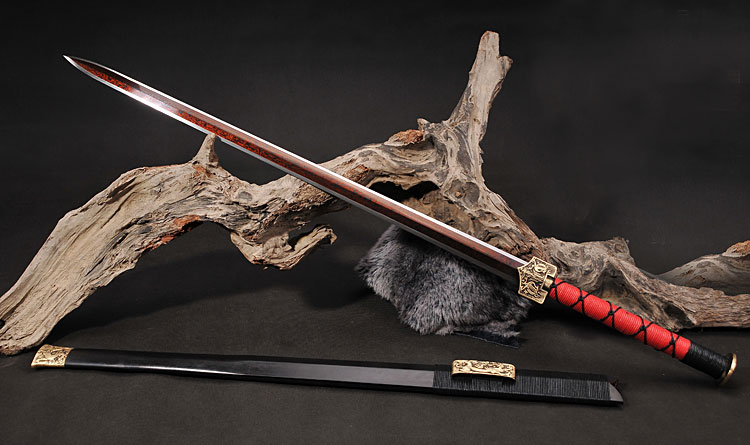
\includegraphics[scale=0.6]{2.jpg}
    \caption{Han Dynasty Sword (劍 - Jiàn) | Image provied by \cite{internalwudangstore_2024_the} }
    \label{fig:enter-label}
\end{figure}

\begin{figure}
    \centering
    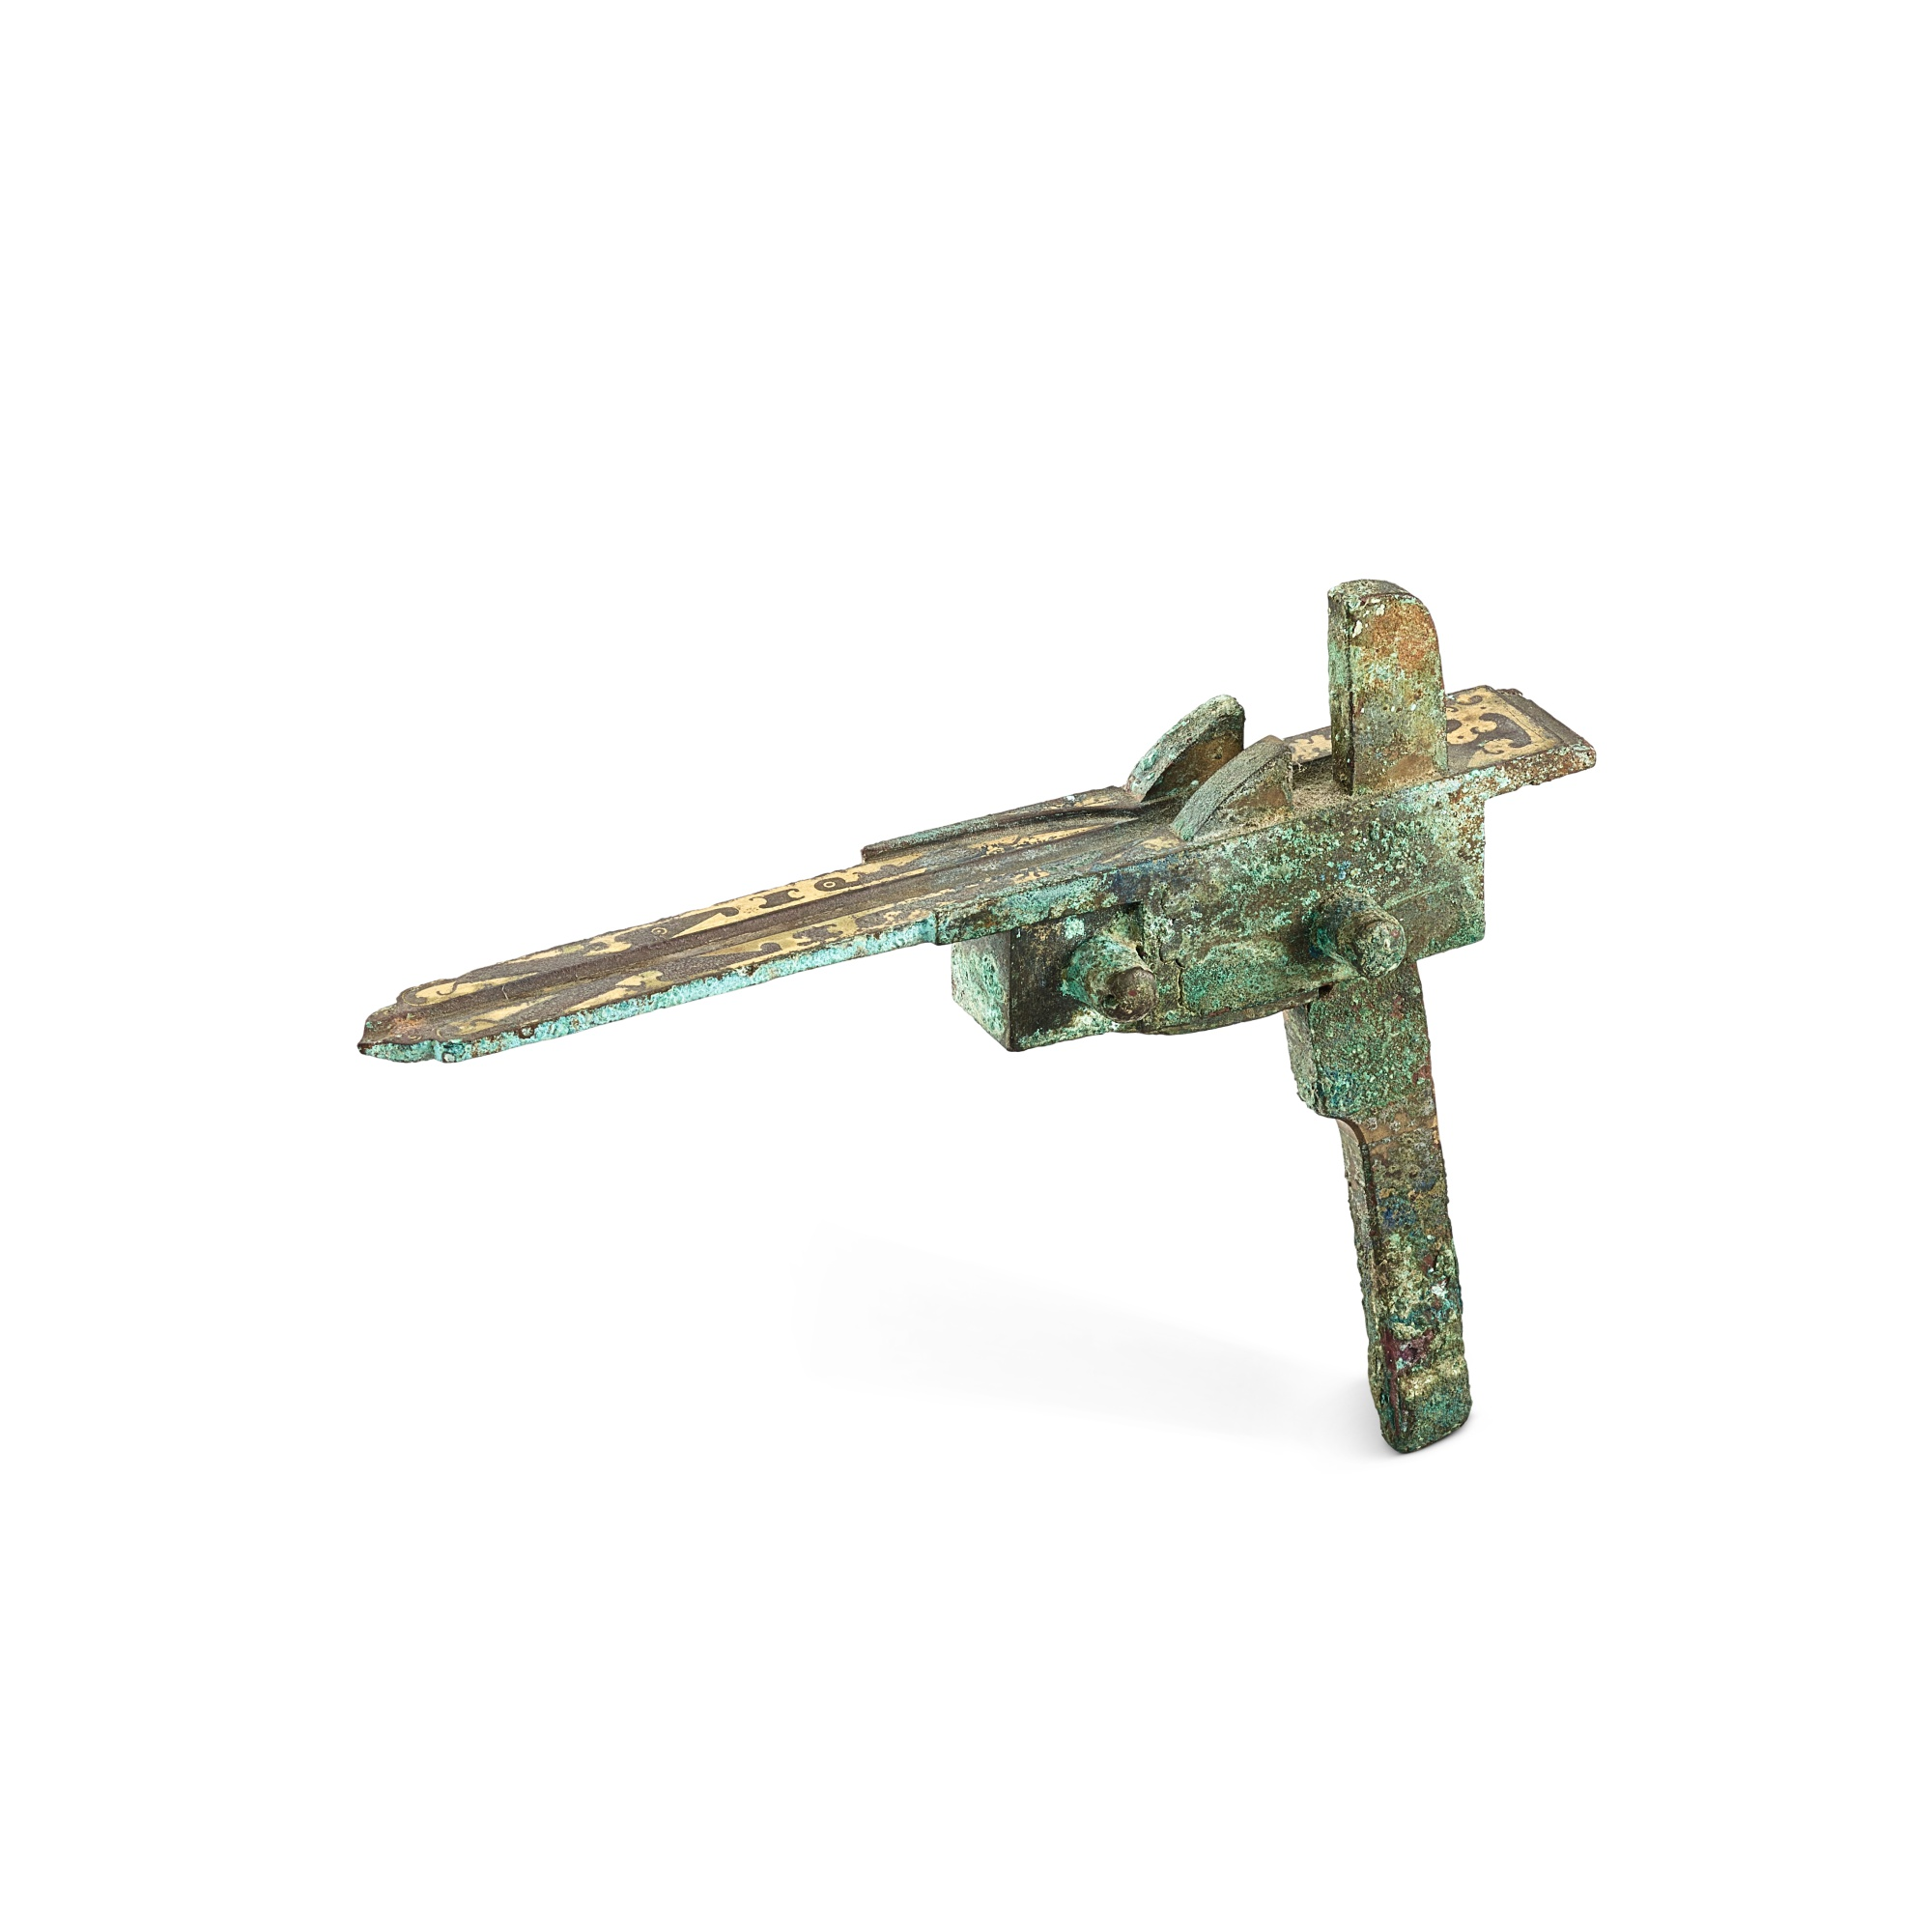
\includegraphics[scale=0.5]{3.jpg}
    \caption{A gold-inlaid bronze crossbow trigger, Han dynasty 漢 銅錯金弩機 from the Gentlemen Collection 士紳收藏}
    \label{fig:enter-label}
\end{figure}
\newpage

\section{Military Strategies Used}
The Han Dynasty’s improved military attacks from the use of stonger and better steel weapons, more advanced crossbows have had a direct impact on military campaigns by the Han, providing them with a stronger edge over their enemies. However, without the use of proper military tactics, the Han Dynasty’s technological advancements would not suffice.

Emperor Wu, who ruled from 141 to 87 BC, was a critical complement for the success of the Han Empire and was responsible for many accomplishments, such as setting up Confucian academies, establishing the Silk Road trade, and keeping the nomadic Xiongnu tribes out \cite{chinahighlights_wudi}. An example of improved strategic planning is shown in the Battle of Mayi (馬邑之圍 - Mǎ yì zhī wéi) in 133 BC during the Han-Xiongnu War. In this battle, Emperor Wu created an army of over 300,000 troops that included infantry, cavalry, and chariot units for an ambush. A spy by the name of Nie Yi feigned defection to the Xiongnu as well as reporting to Junchen Chanyu, the current ruler of the Xiongnu, that the city of Mayi was willing to surrender. This gave the Xiongnu army a sense of relief since they knew they had the advantage, but as soon as Xiongnu Chanyu entered Mayi, the group of 300,000 troops would encircle the army, leading to a successful ambush as they encircled the Xiongnu Chanyu forces \cite{paludan_1998_chronicle}. In this example, it is evident that Emperor Wu’s strategic use of deception and his army were essential to creating a successful ambush of the Xiongnu Army; such tactics show the importance of strategy in Han military success \cite{chineseuniversityofhongkong_the}\cite{msw_2019_the}.

The long term impact of Han military innovation is evident in archaeological findings; recent excavations of Han military sites have revealed tombs that house numerous weapons and military equipment, indicating the advanced technology that the Han military had. Research from Sheng et al (2023). shows that the Picea tree was used by Shichengzi’s planners, a Han Dynasty subsidiary; this provides clear evidence for the usage of timber strategies along the north-western populus of the Han Empire \cite{sheng_2023_wooduse}. In total, the Han Dynasty’s technological and tactical advancements have proved to have a significant effect equally on contemporary military campaigns and long-term development of military strategies in China\cite{ven_2021_warfare}.

\begin{figure}
    \centering
    
\includegraphics[scale=0.45]{1.jpg}
    \caption{Illustration of the Battle of Mayi. Han soilders on the right with black iron armour and on horses (right), while Xiongnu forces on the ground (left) | Provided by \cite{inews_2024_the}.}
    \label{fig:enter-label}
\end{figure}

\section{Influence of Confucian Principles on Han Military Decision-Making}
Confucianism emphasises moral virtue, proper conduct, and social harmony, which had a pronounced impact on shaping the governance and military strategies of the Han Dynasty. Confucianism first started in China and would later influence Korean, Japanese, and Vietnamese societies. Confucius’s principles were righteousness (義 - Yi), humanity (人性 - Rénxìng), and loyalty (忠誠 - Zhōngchéng), which were a dominant part of the decision making process of Han generals and officials \cite{csikszentmihalyi_2024_confucius}. 

Confucianism had emphasized that rulers and military leaders should act with morality and altruism. This principle influenced Han military leaders to prioritise morality and the welfare of their soldiers and civilians. This also played a part in the Han Military Code, where Confucian values encouraged discipline, respect for authority, and a sense of duty among fellow soldiers, displaying qualities such as courage, wisdom, and compassion.

The applications for military cases were evident when Emperor Wu of Han justified his military campaigns against the Xiongnu by linking it to the confuscious value of righeous value by explaining it was to protect the Chinese people and secure their own borders. These campaigns required Han commanders to uphold Confucian values, conduct themselves honorably, and ensure that their actions served the greater good. The Great Wall of China is also an example of this, as it emphasised Confucian values of protection and stability \cite{nylan_2001_the}.

Confucian principles played a central role in how the Han military made its decisions. By incorporating moral and ethical considerations into their strategies, Han leaders ensured their actions were not only effective but also aligned with the principles of social harmony and righteousness. These general ethics not only legitimised their military campaigns but also influenced any future Chinese civilizations, influencing the further development of military thought and practice \cite{dubs_1938_the}.

\section{Final Words}
The influence of the Han Dynasty on ancient weaponry, military tactics, and decision making has been preserved through their advanced use of iron and steel weapons, the sophisticated use of crossbows, and their development of tactical operations, which has provided the Han military with an upper hand against their rivals, particularly against the Xiongu. These innovations have given the empire military success and also laid the groundwork for how well planned strategies can be used to secure their borders and expand their influence.

A major shift in the way the Han military functions has resulted from the Han Dynasty's adoption of Confucian principles. With their strong emphasis on disciplined warfare, morality and the security of their military and civilians it was possible for the Han Dynasty to be a dominant power but also an inspiration for following generations, leaving them a foundation to build their own societies from, leaving a lasting military and philosophical impression 

\section{Acknowledgements}
The author would like to thank the contributions of Aaron Zhao and Professor Barbierie from the University of South Carolina at Beaufort for their substantial contributions and help throughout this historical investigation.

The author would also like to thank Professor Sanft from the University of Tennessee, Knoxville, Dr. Wing-Lun from the UNSW Sydney School of Humanities \& Languages, Professor Meyer-Fong from Johns Hopkins University, and Professor Lo from University College London for their helpful insights into this topic.


% % in case of needing citations
\newpage
\section{References}
\bibliography{refs.bib}

\end{document}
